\documentclass[12pt]{article}

\usepackage[a4paper, top=2.5cm, right=2.5cm, bottom=2.5cm, left=2.5cm]{geometry}
\usepackage{listings}
\usepackage{setspace}
\usepackage{graphicx}
\usepackage{tikz}
\usetikzlibrary{matrix}

\onehalfspace
% Later references:
% - https://pages.cs.wisc.edu/~horwitz/CS704-NOTES/1.LAMBDA-CALCULUS.html
% - https://en.wikipedia.org/wiki/Lambda_calculus
% - https://en.wikipedia.org/wiki/De_Bruijn_index

\title{A lambda calculus compiler}
\author{Áron Hárnási \\
    \normalsize Eötvös Lóránd University, Faculty of Informatics}

\lstdefinestyle{mystyle}{
    basicstyle=\ttfamily,
    frame=lines,
    numberstyle=\small
}

\lstset{style=mystyle}

\begin{document}
\linespread{1}
\maketitle
\pagebreak
\tableofcontents
\pagebreak

\section{Introduction}

This is the user and development documentation of a compiler that compiles a
language inspired by simply typed lambda calculus and produces C source code.

\subsection{Motivation}

Most, if not all languages are based on lambda calculus, however it is not
widely understood. This project is an attempt to gain insight on how functional
languages are translated to imperative code, as well as to outline some of the
difficulties of writing a type system based on simply typed lambda calculus.

\subsection{Terminology}

The name of the compiler described in this document is referred to by the name
\verb$lcc$, while its source language is named LC, or the LC language. It is
important to make the distinction between lambda calculus and the LC language,
as the LC language is designed to be evaluated using physical hardware with
limited resources, and as a result, LC has features that are not present in
lambda calculus and vice versa.

\subsection{Lambda calculus}

Lambda calculus is a mathematical system in which we are able to define any
computation that can be defined with a Turing machine. This is achieved using
function application and substitution on lambda terms. A lambda term in the
simplest form of lambda calculus is built up of three parts:
\begin{itemize}
    \item $(x)$ A variable that can hold a value.
    \item $(\lambda x. F)$ A lambda that can represent a function, where $x$
        is the function parameter and $F$ is another term, that may or 
        may not contain $x$.
    \item $(f\:a)$ A function application where $f$ is the function $a$ is
        applied to. Both $f$ and $a$ are terms. \\ \textbf{Note:} Since variable
        terms can also be denoted with a string of characters, it is important
        to put a space between the two terms to distinguish between a function
        application and a variable term.
\end{itemize}
The main reduction operation is $\beta$-reduction. With $\beta$-reduction, we
can reduce a function application from the form $(\lambda x. F)\:A$ to the
form $F[x := (A)]$, where the $F[x := (A)]$ denotes a new term that is the same
as $F$ except each $x$ variable is replaced with the $(A)$ term.

$\beta$-reduction in this form, can introduce naming collisions in the system.
For example, the term $((\lambda x. (\lambda y. x)) y) z$ would reduce to
$(\lambda y. y) z$ and then $z$. If we instead used $w$ for the parameter of the
inner lambda, $((\lambda x. (\lambda w. x)) y) z$ would reduce to $(\lambda w.
y) z$ and then $y$, which is different from the first scenario.

In order to avoid naming collisions, we can use the $\alpha$-reduction rule.
With $\alpha$-reduction, we can rename variables in a given lambda calculus
term. Renaming can be used before a $\beta$-reduction, for example, in the
previous example $((\lambda x. (\lambda y. x)) y) z$ replacing $y$ with $w$ in
the inner lambda term will result in $((\lambda x. (\lambda w. x)) y) z$, which
does not have naming collisions.


\subsection{This implementation} % todo: split and move to user and dev doc

In this section, we will touch on the most important differences between the
formal system of lambda calculus, and this implementation. There have been some
ideas borrowed from C, Rust, and Haskell in order to make the language usable
from a non-theoretical standpoint.

\subsubsection{Global variables} % todo: split and move to user and dev doc

In order to make the language more usable, much like in Haskell, it is possible
to create global definitions for terms, that can be used in other parts of the
program. This introduces recursion as the main fix-point combinator.

\subsubsection{Static typing} % todo: split and move to user and dev doc

It was decided, that the code this compiler compiles from was going to be
statically typed. Each term has a type that is assigned to it at compile time by
a type inference algorithm. Types of global variables can also be specified, in
which case the compiler checks if it matches the inferred type of the same
variable.

\pagebreak
\section{User documentation}

\subsection{The goal of the project}

The main goal of the project is to implement a compiler for a language based on
simply typed lambda calculus. It should be able to infer as well as check the
types of expressions. Resource and time limitations aside, the language should
be Turing-complete. Additionally, the language should have some way of
communicating with the outside world and therefore some input-output system is
necessary.

\subsection{Methods used} % todo

\subsubsection{Garbage collection}

There is a simple garbage collection algorithm built into the runtime of the
generated code. The algorithm uses a mark-and-sweep style method to find and
free allocated memory that is not used.

\subsubsection{C back-end}

The target language of the compiler is C. There are types and functions in the
LC language that use the C definitions, for example, all number types and
input-output functions.

\subsubsection{Impure functions}

The LC language solves input and output with impure functions, as they make
troubleshooting programs easier. Allowing impure functions also makes
implementation easier, as pure IO functions require a more complex type system.

\subsubsection{Recursive functions}

The language is eagerly evaluated, however for recursion to work, LC is required
to have lazily evaluated constructs. The two main ways to get lazy evaluation,
are if-expressions, and the \verb$case$ function, both of which can be used for
recursion.

\subsection{Building the software}
\subsubsection{Dependencies}

To build the program, one would require the following packages:
\begin{itemize}
    \item git
    \item stack v2.11.1 or later
    \item ghc v9.4.8 or later \\ Note that with default settings, stack usually
        downloads the appropriate ghc version for the project.
\end{itemize}
Note that the compiler was only tested on a few Linux distributions; all of them
on the x86\_64 architecture, and it is possible that it does not work properly
on some others. Using Ubuntu 22.04 should work. It is also recommended, that the
Haskell tools are installed via ghcup. Alternatively, the repository is also set
up to be built on NixOS, which might be a better choice in case it fails on
Ubuntu.

\subsubsection{Compilation and installation}

If all the necessary dependencies are present, building the project should only
require two steps. To build the project, execute the following commands in an
appropriate directory.
\begin{lstlisting}
$ git clone --depth=1 \
    https://github.com/ConcreteCactus/lcc.git
\end{lstlisting}
This will clone the repository, which is hosted on GitHub. In order to build and
install the compiler, one would run the following:
\begin{lstlisting}
$ cd lcc
$ stack install
\end{lstlisting}
This will build and install the required dependencies, including ghc. The
compiler binary is usually copied to \texttt{\$HOME/.local/bin}. Please, make
sure the resulting binary is on the \texttt{PATH}. If the installation goes
correctly, running \texttt{lcc -v} should show a banner similar to the
following:

\vspace{1em}\noindent\begin{minipage}{\textwidth}
\begin{lstlisting}
$ lcc -v
lambda_compiler v1.0

___
\_ \
  \ \       __     __       __     __
   \ \     (_ \   / _)     (_ \   / _)
   /  \      \ \_/ /         \ \_/ /
  / /\ \      ) _ (           ) _ (
 / /  \ \   _/ / \ \_       _/ / \ \_
/_/    \_\ (__/   \__) (_) (__/   \__)
\end{lstlisting}
\end{minipage}

\subsubsection{Runtime dependency}

In order to compile an executable, \texttt{lcc} uses \texttt{gcc} by default.
Therefore it is recommended, to have an installed version of \texttt{gcc} on the
\texttt{PATH}. The version \texttt{lcc} was tested with was gcc v11.4.0, however
it is likely that compilation works on older versions as well. Alternatively, it
is possible to specify a different C compiler with command-line arguments, which
will be discussed under Command-line options.

\subsection{Running the compiler}

The main job of the compiler is converting from LC source code to C source code.
Once it has the C source file, it is compiled to binary using \texttt{gcc} if no
other command-line option is specified. The file extension of the input file
does not matter, however in this document they will be referred to with the
extension \texttt{.lc}. To simply compile an input file, one would run the
following:
\begin{lstlisting}
$ lcc hello.lc
\end{lstlisting}
This command compiles the input file \texttt{hello.lc} and produces a binary
file with the default name \texttt{gcc} gives to output binaries. On Linux it is
usually \texttt{a.out}. \texttt{lcc} produces a \texttt{.c} file containing the
source code it has generated as well with the default name \texttt{a.c}.

\subsubsection{Command-line options}

It is possible to give command-line options to the compiler in order to alter
its behavior. 

\vspace{7pt}

\begin{tabular}{l l}
    \texttt{-n}\quad& Do not run any C compiler, only compile from \\ 
                    & LC to C. \\
    \texttt{-v}\quad& Show version and about information and exit. \\
    \texttt{-h}\quad& Print some help text and exit. \\
    \texttt{-o <output-exe>}\quad& Specify the name of the executable
        generated. \\
    \texttt{-O <output.c>}\quad& Specify the name of the C source generated. \\
    \texttt{-c <cc>}\quad& Specify the C compiler command.
\end{tabular}

\vspace{8pt}

\textbf{Note:} When using \texttt{-n} and \texttt{-o} and/or \texttt{-c} together,
no C compiler will be run. Also note that when using \texttt{-v} or \texttt{-h},
no compilation of any kind will be performed. 

\subsection{The LC language}

The LC language is a language inspired by simply typed lambda calculus.
Expressions are similar to lambda calculus terms, they are simply typed, and
types support parametric polymorphism. In this subsection, the key details of
the language will be discussed.

\subsubsection{Syntax and semantics}

Syntactically, the language has several similarities to Haskell. Global
variables can be defined with the \texttt{:=} operator in the following way.
\begin{lstlisting}
globalVariable := expression
\end{lstlisting}
Optionally, a type wish or declaration can be added to a global definition,
(i.e., its intended type can be specified.) For each type wish, the compiler
checks if it can be used in place of the inferred type. To specify a type wish,
one can use the colon (\verb$:$) operator in the following way:
\begin{lstlisting}
globalVariable : I32 -> I32 -> I32
globalVariable := expression
\end{lstlisting}
In this case, \verb$globalVariable$ is a function that takes two 32bit signed
integer parameters, and outputs a 32bit signed integer.

\subsubsection{Expressions}

All expressions can be created using six parts:
\begin{itemize}
    \item Variables
    \item Lambdas
    \item Applications
    \item Global references
    \item If expressions
    \item Literals
\end{itemize}

\paragraph{Variables} Variables always represent function parameters. They can
be denoted with a single ASCII character, or a string of ASCII characters. Their
first character is always lower-case. For example, \verb$x$ or \verb$exampleVar$.

\paragraph{Lambdas} Lambdas represent functions. Lambdas have an expression
body, and a parameter. Their parameter can be used inside their expression
body. To create a lambda, one would write a backslash (\verb$\$) character
followed by the parameter name, a dot (\verb$.$), and the expression body. For
example, \verb$\x.x$ or \verb$\a.(f a) g$.

\paragraph{Applications} Applications represent calling functions. Applications
always contain two expressions, The first of which is the function getting
called and the second represents the parameter given to that function. To apply
an expression to another in the LC language, one would write the function to be
called first and the parameter second separated by white-space. For example,
\verb$func param$ or \verb$func param1 param2$.
\noindent
Note that function application is left-associative.

\paragraph{Global references} Global references denote expressions defined
somewhere else in the file. When evaluated, these references are
substituted\footnote{On the compiler level, this substitution is implemented as
    a function call, which happens in a new scope; therefore it is not possible
    to have, for example, free variables in global definitions.} with the
corresponding global definitions. Global references are written in the same way
as local variables; therefore in name-collisions, the local variable will take
precedence.

\paragraph{If expressions} If expressions represent the control-flow if
primitive used in procedural languages. If expressions take three expressions:
one that evaluates to a boolean, one that is used when the boolean is true, and
one that is used when the boolean is false. If expressions are lazy, which makes
it possible to use them in recursive functions when other lazy constructs are
not available or necessary. \\
For example, \verb$if condition then exprIfTrue else exprIfFalse$

\paragraph{Literals} Literals represent number values in the C back-end, and the
standard library provides basic operations on them. The following table shows
the possible types they can have and their corresponding C type in the LC
language.
\begin{center}
\begin{tabular}{c c c}
    LC type & Type postfix & C type \\
    \hline
    \verb$I8$ to \verb$I128$ & \verb$i8$ to \verb$i128$ & \verb$int8_t$ to
    \verb$int64_t$ and \verb$__int128$ \\
    \verb$U8$ to \verb$U128$ & \verb$u8$ to \verb$u128$ & \verb$uint8_t$ to
    \verb$uint64_t$ and \verb$unsigned __int128$ \\
    \verb$F32$ and \verb$F64$ & \verb$f32$ and \verb$f64$ & \verb$float$ and
    \verb$double$ \\
    \verb$USize$ & \verb$usize$ & \verb$size_t$ \\
    \verb$Char$ & \verb$char$ & \verb$char$ \\
    \verb$Bool$ & \verb$bool$ & \verb$bool$
\end{tabular}
\end{center}
There are four different ways to write literals. To write a character literal,
one would write the desired character between two single quotes. Escape
sequences are not supported. For example, \verb$'a'$ or \verb$' '$.

With the exception of characters, in the LC language, it is required to use a
type specifying postfix when writing literals. To write a hexadecimal number,
one would prefix it with \verb$0x$ and write the desired value with the
characters \verb$0$-\verb$9$ and \verb$a$-\verb$f$. Hexadecimal numbers need to
be postfixed with an underscore (\verb$_$) and the desired type postfix shown in
the table above. Only unsigned integers, characters, and booleans can be written
in this form. For example, \verb$0x1_u8$ or \verb$0xdeadbeef_u32$.

In order to write a floating point number, one would write the whole part of the
number in decimal form, optionally include the fractional part separated by a
dot (\verb$.$) character, then write the postfix \verb$f32$ or \verb$f64$. For
example, \verb$0f32$ or \verb$3.14f64$.

Decimal numbers can be written similarly to floating point ones with the
exception that decimal numbers can not have a fractional part. Decimal numbers
can be postfixed with all type postfixes except \verb$f32$ and \verb$f64$. For
example, \verb$42u32$ or \verb$-1i8$.

\subsubsection{Types}

The LC language is statically typed. This means, that all expressions have a
set type at the end of compilation. The language uses a type inference algorithm
that runs on all expressions to determine the appropriate type for each
expression. Because of type inference it is not required for the programmer to
specify the type of expressions; however, types of global definitions can still 
be specified for clarification.

When a type is specified for a global definition, the type checker is run. The
type checker compares the specified type and the inferred type to see if they
are in line with each other. If the types match, the specified type is used in
place of the inferred type. By default, the type inference algorithm tries to
find the widest possible type for a given expression, and the type found by the
inference algorithm can be narrowed down by specifying the type if desired. For
example, the following program compiles:
\begin{lstlisting}
f1 := \x.x
main := f1 0i32
\end{lstlisting}
while the second one returns a type checker error:
\begin{lstlisting}
f1 : I8 -> I8
f1 := \x.x
main := f1 0i32
\end{lstlisting}
In this example, the type of the \verb$f1$ function was narrowed down when its
type was specified, and the compiler rejected the expression that tried to apply
a parameter to the \verb$f1$ function that was outside of its possible parameter
types.

In the next paragraphs, the key components of the type system are discussed. All
types in the language can be one of the following kinds:
\begin{itemize}
    \item Atomic types
    \item Function types
    \item Generic types
    \item Sum types
    \item Product types
    \item List types
    \item The Unit type
    \item The Empty type
\end{itemize}

\paragraph{Atomic types} Atomic types are the types whose elements are the
language primitives. For example, \verb$I32$ or \verb$Char$. All language
primitives can be constructed using literal expressions discussed in the
previous subsection. For a list of possible atomic types, the table shown in the
Literals paragraph can be used.

\paragraph{Function types} Function types are the types of functions. The
elements of function types can be constructed using lambda expressions, while
the function types themselves can be constructed with the arrow (\verb$->$)
operator. In order to construct a function type, the parameter type is written
first and the return type is written second infixed with the arrow operator. The
arrow operator is right-associative. For example, \verb$I32 -> Char$ or 
\verb$U8 -> a -> a$.

\paragraph{Generic types} Generic types allow function types to be generalized
to work with any parameter type. They denote that the type of the parameter does
not matter for the implementation of the function. There are no constructors for
generic types, as they are not concrete types. When expressions with a concrete
type are applied to a function with a generic type for a parameter, the generic
type of the function is substituted for the concrete type of the expression. To
specify generic types, one can use any string of alphanumeric characters so long
as it starts with a lowercase letter. For example, \verb$a$ or
\verb$genericType$.

\paragraph{Sum types} Sum types are types that have two kinds of elements:
\emph{left} and \emph{right}. \emph{Left} elements always contain an element of
one type, while \emph{right} elements always contain an element of a different
type. To specify a sum type with type \verb$A$ and \verb$B$ as \emph{left} and
\emph{right} types, one would use the plus-sign (\verb$+$) operator in the
following way: \verb$A + B$.

The standard library provides two constructors for sum types; one that
constructs \emph{left} elements: \verb$inl$, and one that constructs
\emph{right} elements: \verb$inr$. Both constructors take one parameter, the
element to be contained. The type of the constructors is the following:
\begin{lstlisting}
inl : a -> a + b
inr : b -> a + b
\end{lstlisting}
Because of this, elements of sum types can either be
\emph{left} or \emph{right} elements. To look into an element of a sum type, one
would use the \verb$case$ function. This function takes three parameters: the
element of the sum type, a function in case it is a left element, and a function
in case it is a right element. The return value of the \verb$case$ function is
the return value of the two functions given to it. The \verb$case$ function has
the following type:
\begin{lstlisting}
case : a + b -> (a -> c) -> (b -> c) -> c
\end{lstlisting}

\paragraph{Product types} Product types are types whose elements contain two
different elements of two different types: a \emph{first} element and a
\emph{second} element. To specify that an expression has a product type with
\verb$A$ and \verb$B$ as the types for its \emph{first} and \emph{second}
elements, one would use the multiplication (\verb$*$) operator in the following
way: \verb$A * B$.

The standard library provides one constructor to create elements of product
types, the \verb$tuple$ function. It takes two parameters and returns an element
of the product type with those parameters.
\begin{lstlisting}
tuple : a -> b -> a * b
\end{lstlisting}
To return back the elements used to construct the product type, there are the
\verb$fst$ and \verb$snd$ functions. \verb$fst$ returns the \emph{first}
element, and \verb$snd$ returns the \emph{second} element.
\begin{lstlisting}
fst : a * b -> a
snd : a * b -> b
\end{lstlisting}

\paragraph{List types} List types are the only recursive datatype in the LC
language as it is not possible to define one using the language primitives. List
can contain a variable number of elements of a single type. To specify a list
type, one can write the type of its elements between two square brackets, for
example, \verb$[I32]$ or \verb$[U8 + Unit]$.

To construct list types, the \verb$emptyList$ and \verb$cons$ functions can be
used. The \verb$emptyList$ function creates a list with no elements, while the
\verb$cons$ function takes an element and a list, and creates a new list with
the element prepended to it.
\begin{lstlisting}
emptyList : [a]
cons      : a -> [a] -> [a]
\end{lstlisting}
To get back the elements used to construct a list, the \verb$uncons$ function
can be used. It takes a list as its parameter, and returns the element of a sum
type which can be used in a \verb$case$ function. The left element of the sum
type can contain a product with the head and tail of the list, while the right
element of the sum type only contains a unit, in case the \verb$uncons$ function
was used on an empty list.
\begin{lstlisting}
uncons : [a] -> a * [a] + Unit
\end{lstlisting}

\paragraph{The Unit type} The unit type is a type that contains one element, and
it can be used mostly to return errors. For example, an array index lookup can
fail if the index given is outside the bounds of the array. When this happens,
the error can be returned using a unit type. In this case, the type of an 
array\footnote{In this document and in the language, the words list and array 
    are used somewhat interchangeably, however to implement the list type, a
    linked-list is used in the back-end.} index lookup function could look
    similar to the following:
\begin{lstlisting}
arrayIndexLookup : [a] -> I32 -> a + Unit
\end{lstlisting}
The function could return an element of a sum type that could either be the
resulting value of the lookup, or the element of the Unit type, meaning that the
function failed.

To construct the element of the unit type, the \verb$unit$ function can be used.
It takes no arguments:
\begin{lstlisting}
unit : Unit
\end{lstlisting}

\paragraph{The Empty type} The Empty type is a type that has no elements. It was
added to the language to make it possible to define statements in zero-order
logic. For example, the statement $A \vee \bot \rightarrow A$ would be defined
with
\begin{lstlisting}
stmt : a + Empty -> a
stmt := \ae. case ae (\a. a) (\e. exfalso e)
\end{lstlisting}
\textbf{Note:} The function \verb$exfalso$ can be used to return an element of
any type if an element of the Empty type is present. (Because there are no
elements of the empty type, this function will never run.)
\begin{lstlisting}
exfalso : Empty -> a
\end{lstlisting}

\subsubsection{Standard library}

The standard library provides functions that let the programmer interact with
the underlying C back-end. The functions it provides can be organized into five
categories:
\begin{itemize}
    \item Arithmetic operators
    \item Comparison operators
    \item Casts
    \item IO functions
    \item Constructors and basic operations on primitives
\end{itemize}

\paragraph{Arithmetic operators} Addition subtraction multiplication and
division operations are implemented in the following standard library functions:
\begin{lstlisting}
add_u8 : U8 -> U8 -> U8
sub_u8 : U8 -> U8 -> U8
mul_u8 : U8 -> U8 -> U8
div_u8 : U8 -> U8 -> U8
...
add_f64 : F64 -> F64 -> F64
sub_f64 : F64 -> F64 -> F64
mul_f64 : F64 -> F64 -> F64
div_f64 : F64 -> F64 -> F64
\end{lstlisting}
In other words the \verb$add_$, \verb$sub_$, \verb$mul_$, and \verb$div_$
functions postfixed with the type postfix are implemented for every type. They
use the usual \verb$+$, \verb$-$, \verb$*$, and \verb$/$ operators in the C
back-end. This means, for instance, that the \verb$div_u8$ function would divide
the same way the C (\verb$/$) operator would. For example, \verb$div_u8 5u8 2u8$
would return \verb$2u8$.

\paragraph{Comparison operators} The following numeric comparison operators are
implemented: $=$, $\le$, $<$, $\ge$, $>$, and $\ne$. In the LC language, they
are named \verb$iseq_$, \verb$isle_$, \verb$islt_$, \verb$isge_$, \verb$isgt_$,
and \verb$isne_$ respectively. Similarly to the arithmetic functions, the
function names are postfixed with the type name they operate on.
\begin{lstlisting}
iseq_u8 : U8 -> U8 -> Bool
isle_u8 : U8 -> U8 -> Bool
islt_u8 : U8 -> U8 -> Bool
isge_u8 : U8 -> U8 -> Bool
isgt_u8 : U8 -> U8 -> Bool
isne_u8 : U8 -> U8 -> Bool
...
\end{lstlisting}
These implementations also use the underlying C comparison operators: \verb$==$,
\verb$<=$, \verb$<$, \verb$>=$, \verb$>$, and \verb$!=$.

\paragraph{Casts} Every primitive type can be cast to every other primitive type
with the casting functions provided by the standard library. The name of every
casting function starts with the name of the type to be cast from, and ends with
the name of the type to be cast to, infixed with the word \verb$To$. For example
the function that casts from \verb$F32$ to \verb$U8$ would be named
\verb$f32Tou8$. All casting functions take a single parameter, the element of
the type to be cast from, and return the element of the type to be cast to.
\begin{lstlisting}
u8Tou16   : U8 -> U16
i32Tou16  : I32 -> U16
f32Tochar : F32 -> Char
...
\end{lstlisting}

\paragraph{IO functions} The IO functions provided by the standard library are
impure functions that enable the program to read from standard in, and write to
standard out. To print to the standard out, one would use one of the
\verb$print_$ functions postfixed with the type of the value to be printed. Not
all primitive types have print functions, namely 128bit types are not supported.

Print functions take two parameters. The first parameter is the value to be
printed to \verb$stdout$ and the second value is the return value, since print
functions do not return any value in the C language. Therefore the type
definition of a print function that prints, for example, characters would be the
following:
\begin{lstlisting}
print_char : Char -> a -> a 
\end{lstlisting}
\textbf{Note:} Print functions only print the given value to the screen once the
second parameter is applied to them.

To read from \verb$stdin$, one can use the \verb$getchar$ function provided by
the standard library. It binds to the \verb$getchar$ function in the C back-end.
Similarly to the \verb$getchar$ function in the C language, \verb$getchar$ in
the LC language returns an integer that, along with the \verb$eof$ function, can
be used to check whether the end of the file is reached.
\begin{lstlisting}
getchar : I32
eof     : I32
\end{lstlisting}
In practice, using \verb$getchar$ can be unintuitive. For example, to write a 
\verb$readfile$ function, one might try to do the following:
\begin{lstlisting}
readfile : [Char]
readfile := if iseq_i32 getchar eof 
    then emptyList 
    else cons (i32ToChar getchar) readfile
\end{lstlisting}
However, using \verb$getchar$ twice in this manner will execute its side-effect
twice as well, which means that the character appended to the character list
will be different from the character used in the if condition. This function
will return only every second character in a file, which is not the expected
behavior.

To overcome this issue, one can define the \verb$let$ function used in some of
the example programs discussed later. The type and definition of the \verb$let$
function is
\begin{lstlisting}
let : a -> (a -> b) -> b
let := \x.\f. f x
\end{lstlisting}
Using \verb$let$ it is possible to capture the return value of the
\verb$getchar$ function to be used multiple times.
\begin{lstlisting}
readfile : [Char]
readfile := let getchar \c. if iseq_i32 c eof 
    then emptyList 
    else cons (i32ToChar c) readfile
\end{lstlisting}
The modified \verb$readfile$ function now returns every character from the
standard input, and not only every second one.

\paragraph{Constructors and basic operations on primitives} Types and the
provided basic functions on them are discussed in the Types subsection;
therefore only the type definitions are shown here.
\begin{lstlisting}
inl       : a -> a + b
inr       : b -> a + b
case      : a + b -> (a -> c) -> (b -> c) -> c
tuple     : a -> b -> a * b
fst       : a * b -> a
snd       : a * b -> b
emptyList : [a]
cons      : a -> [a] -> [a]
uncons    : [a] -> a * [a] + Unit
unit      : Unit
exfalso   : Empty -> a
\end{lstlisting}

\subsubsection{A note on white-space}

To break an expression down into multiple lines, one would insert end of line
characters inside the white-space between expression parts. Lines that are part
of a previous expression have to start with some sort of white-space, in order
for the compiler to differentiate between continued expressions and new
definitions.
\lstset{showspaces=true}
\begin{lstlisting}
adder := \a. \b.
 add_i32 a
         b
nextDefinition := nextExpression
\end{lstlisting}
\lstset{showspaces=false}

\subsubsection{The main function}

When a program compiled by \verb$lcc$ starts, the \verb$main$ function is
evaluated. Since the return value of the main function is used as the exit code
of the program, the main function can only have type \verb$U8$.

It is allowed to compile a program without a main function, however running the
resulting binary will simply exit with exit code 0.

\subsubsection{Compilation errors}

The compiler can show an error message in case the program has errors. The error
message contains the line and column number of the position the error was found
on. The precision of the position depends on the type of the error, which
there are three of:
\begin{itemize}
    \item Syntactic and lexical errors
    \item Semantic errors
    \item Type errors
\end{itemize}

Syntactic and lexical errors show the position the error was found at, while
semantic and type errors only show the start of the declaration or definition
the error was found at.

\paragraph{Syntactic and lexical errors} Syntactic and lexical errors are
reported with the message \verb$lexical error$. These errors can occur due to
the following reasons:
\begin{itemize}
    \item Mistyped operators (e.g. \verb$=$ instead of \verb$:=$)
    \item Mismatched brackets 
    \item Bad syntax (e.g. \verb$\x x$ instead of \verb$\x.x$)
\end{itemize}

\paragraph{Semantic errors} Semantic errors are reported with the message
\verb$semantic error$. Semantic errors can only occur in syntactically correct
source codes. Semantic errors can be one of the following:
\begin{itemize}
    \item When a global variable is redefined.
    \item When the type wish of a global variable is redefined.
    \item When there is a reference to an undefined global variable. 
\end{itemize}

\paragraph{Type errors} Type errors are reported with the message
\verb$type error$. Type errors can only occur in semantically correct source
codes. A type error can have one of the following kinds:
\begin{itemize}
    \item When the type of an expression could not be inferred due to a self
        reference.
    \item When two types could not be matched.
    \item When a type wish did not match the inferred type of an expression.
    \item When a value is applied to an expression whose type is not a function.
    \item When a condition of an if expression is not a boolean.
\end{itemize}

\subsection{Example programs}
\lstset{numbers=left}

In this section, some example programs will be discussed, so that it is easier
to understand the language.

\subsubsection{A Hello World program}

A simple hello world program would be the following:
\lstinputlisting{../examplePrograms/hello.lc}

When run, this program would print the string \verb$hello world$ to the standard
output, then exit. In order to write a string of characters to the standard
output, one would need to first define a function that can take a list of
characters, and compose a new function that prints the characters in the list
one by one. This is the task of the \verb$printList$ function.

The \verb$printList$ function first does a case study on the head of the list.
If the list is not empty, the first element is printed, then \verb$printList$ is
called recursively on the remaining list. If the list is empty, the identity
function is returned to align with the type of the \verb$printList$ function.

\verb$cmp$ is a small utility function that returns the composition of the two
input functions flipped. It is used in the \verb$printList$ function to compose
the character printing function first and the recursive call second.

\verb$hello$ is simply the list that gets printed. Since the LC language does
not support list literals, the list is constructed with the repeated use of the
\verb$cons$ function.

\subsubsection{A Single-digit calculator}

The next example program is a calculator. For simplicity, the calculator can
only do arithmetic on single decimal digits.

\lstinputlisting{../examplePrograms/sdc.lc}

The most important functions in the above program are \verb$readDigit$ and
\verb$doCalc$. \verb$readDigit$ reads a single character from the standard
input, and returns a value that is either the digit read, or a unit meaning that
the read digit was not in the 0-9 range. For simplicity, the program assumes
that it is not the end of the file when reading characters.

\verb$doCalc$ takes three parameters: the two numbers to do an operation on, and
a character that is the operator between the two numbers. The function then
checks whether the character is any of the four basic arithmetic operators:
\verb$+$, \verb$-$, \verb$*$, and \verb$/$. If it is, the function returns the
result of the corresponding arithmetic operation inside a sum type. If the
character could not be matched to one of the known operators, the function
returns a unit that shows that an error has occurred.

The \verb$main$ function uses the \verb$readDigit$ and \verb$doCalc$ functions,
checks if any of them returns an error, and prints the result of the
\verb$doCalc$ function if there are no errors. If instead there are any errors,
the main function does not print to the standard output, instead it exits with
the exit code 1, meaning the operator was not recognized; 2, meaning the second
digit was not in the 0-9 range; 3, meaning the first digit was not in the 0-9
range.

\subsubsection{A Turing-machine simulator}

One way to show that a programming language is Turing-complete is to show that
it can simulate a Turing machine. A program in the LC language that simulates a
Turing machine can be found under \verb$examplePrograms/turing.lc$. The source
code is not included in this document as it is quite long.

The simulator reads in two lines. One for the state transitions of the Turing
machine, and one for its input. The state transitions are encoded with ones and
zeroes in the following way:
\lstset{frame=none}
\lstset{numbers=none}
\begin{lstlisting}
<cell>11<cell>11<cell>11...11<cell>
\end{lstlisting}
Where each \verb$<cell>$ defines one state transition. To encode more than one
cell, one would need to separate them with two ones.

A \verb$<cell>$ can be encoded in the following way:
\begin{lstlisting}
<state>1<read>1<next state>1<write>1<direction>
\end{lstlisting}
Where \verb$<state>$ is the current state, \verb$<next state>$ is the state to
transition to, \verb$<read>$ is the symbol read from the tape, \verb$<write>$ is
the symbol to be written to the tape, and \verb$<direction>$ is the direction
the head should move. All five of these values can be encoded with one or more
repeating zero characters.

There are three special \verb$<state>$ values. The start state, which can be
encoded with a single \verb$0$ character, is always the state the machine starts
with in the beginning of its execution. The accept state, that can be encoded
with \verb$00$ is the state the machine should transition to if it accepts the
input. The reject state, that can be encoded with \verb$000$ is the state the
machine should transition to when it rejects the input. Both the accept and
reject states are halting states, which means that transitioning to either of
them ends the execution. All other states can be used without any special 
restriction.

Both the \verb$<read>$ and \verb$<write>$ values encode symbols that can be on
the tape including the empty symbol, a symbol that the tape is filled with
before the input is loaded. The empty symbol can be encoded with a single
\verb$0$. This \verb$0$ is different from an input \verb$0$ character, since the
input can not contain empty symbols. To encode a \verb$0$ character, one needs
to use \verb$00$ and to encode a \verb$1$ character, one needs to use
\verb$000$. Other symbols can be used with four or more consecutive zeros,
however the simulator might not be able to display them properly.

The \verb$<direction>$ field can have three values. These three values encode
moving left, moving right, and not moving. \verb$0$ can be used to encode moving
left, \verb$00$ can be used to encode not moving, and \verb$000$ can be used to
encode moving right.

After receiving the first line, the Turing machine simulator parses the input,
and either prints an \verb$e$ character indicating that there was an error while
parsing, or it prints the defined state transitions one by one in a human
readable way. Note that the machine allows undefined state transitions. During
execution when it does not find the proper state transition for a specific state
and symbol combination, it prints \verb$E2$ and stops execution.

After the second line is read, the machine loads the input onto the tape and
starts execution. Each step of the execution is printed to standard output with
the current state, tape, and head position.

\lstset{frame=lines}

An example input to the Turing machine can be found in the repository at\\
\verb$examplePrograms/turing_input.txt$. The file is written in a way to allow
being piped into the simulator itself. To run the simulator with the example
input, one can compile its source with
\begin{lstlisting}
cd examplePrograms
stack run turing.lc
\end{lstlisting}
The command creates a \verb$a.out$ executable file, that can be used to run the
simulator. To run the simulator with the given example input directly, one might
pipe the contents of the file into the program. On \verb$bash$ that is done in
the following way:
\begin{lstlisting}
./a.out < turing_input.txt
\end{lstlisting}
The program should then print the state transitions and the execution of the 
simulated Turing machine:
\begin{lstlisting}
q0 _ :> q1 _ --
q0 0 :> q3 _ ->
q0 1 :> q4 _ ->
q3 0 :> q3 0 ->
q3 _ :> q5 _ <-
q3 1 :> q3 1 ->
q4 0 :> q4 0 ->
q4 1 :> q4 1 ->
q4 _ :> q6 _ <-
q5 0 :> q7 _ <-
q5 _ :> q1 _ --
q5 1 :> q2 1 --
q6 1 :> q7 _ <-
q6 0 :> q2 0 --
q7 0 :> q7 0 <-
q7 _ :> q0 _ ->
q7 1 :> q7 1 <-
\end{lstlisting}
This Turing machine accepts the input if it only consists of ones and zeroes,
and it is symmetrical. If the input is not symmetrical, the Turing machine
rejects the input. Note that there are some undefined state transitions.

The execution of the Turing machine is the following. Note that some lines have
been removed to keep the output concise.
\begin{lstlisting}
q0 0 > 0 0 1 0 1 0 0 0 
q3 1 > _ 0 1 0 1 0 0 0 
...
q3 8 > _ 0 1 0 1 0 0 0 _ 
...
q7 6 > _ 0 1 0 1 0 0 _ _ 
...
q3 2 > _ _ 1 0 1 0 0 _ _ 
...
q7 5 > _ _ 1 0 1 0 _ _ _ 
...
q4 3 > _ _ _ 0 1 0 _ _ _ 
...
q2 5 > _ _ _ 0 1 0 _ _ _ 
\end{lstlisting}
The result of the execution can be read out from the last state of the Turing
machine: \verb$q2$. In this case, it has rejected the input because it was not
symmetrical.

\lstset{numbers=left}

\pagebreak
\section{Developer documentation}

This part of the documentation is intended for developers of the compiler, and
users of the language should not need to use it.

\subsection{Project structure}

The compiler can be broken down into four parts: Lexer, Syntax checker, Semantic
analyzer, and Code Generator. These four parts represent the four steps in
compilation, which will be discussed in detail in the following sections.

\begin{figure}[h]
\includegraphics[width=0.8\textwidth]{high-level-architecture.diag.pdf}
\centering
\caption{High level modules in the compiler.}
\end{figure}

\subsubsection{Folder structure}

Most modules in the repository have two files: An internal one that exports all
external and internal functions and an external one that imports the internal
file, and only exports the external functions. When this module is imported into
other modules, the external file is used. In order to unit test the internals of
a module, it is necessary to expose them to unit tests. Using this two file
structure allows the proper encapsulation of internal functions, while it also
enables the programmer to test the module, as in unit tests the internal file
can be imported.

\lstset{numbers=none}
\begin{lstlisting}
src/
|-MyModule/
  |-Internal.hs -> All definitions
|-MyModule.hs -> Exposes external functions
\end{lstlisting}

\subsection{Lexer and Syntax checker}

\begin{figure}[t]
\includegraphics[width=0.8\textwidth]{syntax-checker.diag.pdf}
\centering
\caption{Module imports related to the Syntax checker}
\end{figure}

When the compiler is invoked, the given source code is loaded into memory as a
\verb$String$. This source code is then used by the Lexer and
Syntax checker to build a syntax tree, which is then given to the
Semantic analyzer for further processing.

\subsubsection{The method of parsing lexical tokens}

The Lexer is responsible for correctly parsing the individual tokens used in the
source code. It defines an applicative functor named Parser that is used
extensively throughout the Lexer and Syntactic analyzer modules. 

The most used functions that can be used to define parsers are the
\verb$satisfy$ and \verb$satify_$ functions. These functions take a predicate on
a character, and return a parser that parses characters for which the predicate
returns true. By chaining together parsers returned by the \verb$satisfy$
functions, it is possible to define parsers for longer strings.

To define a parser for a lexical token, the \verb$satisfy$ and \verb$satisfy_$
functions are used along with the \verb$Applicative$ and \verb$Alternative$
utility functions, for example, \verb$some$, \verb$many$, and the \verb$<|>$
(alternative) operator. These primitives allow the creation of regex-like
parsers, for example, the parser for hexadecimal number literals is defined in
the following way:
\\\noindent\begin{minipage}{\textwidth}
\begin{lstlisting}
( satisfy_ (== '0')
    *> (satisfy_ (== 'x') <|> satisfy_ (== 'X'))
    *> some (satisfy isHexDigit)
    <* satisfy (== '_')
) <*> litPostfix unsignedIntAtomicTypes
\end{lstlisting}
\end{minipage}
First, the \verb$0$ and \verb$x$ characters are parsed allowing upper and
lowercase \verb$x$ characters. Then, one or more hexadecimal digits ending with
an underscore are parsed. Because hexadecimal literals need to be postfixed with
a type postfix, the postfix is parsed using the \verb$litPostfix$ function. This
example also shows that hexadecimal literals can only encode unsigned integers.

\subsubsection{The structure of the Syntactic analyzer}

The main goal of the Syntactic Analyzer is to process the input string using the
tokens defined in the lexer, return a syntax-tree to be used in the semantic
analyzer, and error on failure. The syntactic analyzer completes most of these
tasks by using the \verb$Parser$ defined in the Lexer.

The Syntactic Analyzer exports the \verb$parseProgram$ function, that directly
turns an input string into either a correct syntax-tree or an error message
depending on whether the input source code was syntactically correct or not. The
type of the syntax-tree is named \verb$Program$, which is an alias for a list of
\verb$ProgramPart$ elements. A \verb$ProgramPart$ contains the name of a global
variable and either a \verb$Declaration$ containing a type wish (or simply
\verb$Type$), or a \verb$Definition$ containing an \verb$Expression$.

All \verb$Program$, \verb$ProgramPart$, \verb$Expression$, and \verb$Type$ have
a corresponding parser defined in the Syntactic Analyzer along with all
constructors of Expression and Type.

\subsection{Semantic analyzer}

Once the syntax-tree is created, the Semantic Analyzer can start processing it.
The Semantic Analyzer is responsible for six tasks:
\begin{itemize}
    \item Assign De-Bruijn indices to function parameters.
    \item Assign incremental indices to generic types.
    \item Check that there are no duplicate or undefined global definitions.
    \item Build a dependency list of the definitions in the order they need to
        be type inferred.
    \item Run the type inference algorithm and apply type wishes.
    \item Check that the \verb$main$ function has the correct type.
\end{itemize}

\begin{figure}[t]
\includegraphics[width=\textwidth]{semantic-analyzer.diag.pdf}
\centering
\caption{Module imports related to the Semantic Analyzer}
\end{figure}

If any of the above tasks fail, an error is produced, and the compilation stops.
If all tasks finish successfully, the processed code is then sent to the Code
Generator, which can start generating the C source code.

\subsubsection{De Bruijn indexing}

One way of eliminating naming collisions is the use of De Bruijn indexing. Bound
variables can be represented not with names given to them at the start of a
lambda term, but instead with numbers denoting how far the variable occurrence
is compared to the lambda term that the variable is bound to. For example, the
term $(\lambda x. (\lambda y. x))$ with De Bruijn indices would be $\lambda
\lambda 2$, or the term $(\lambda y. (\lambda z. ((\lambda x. (\lambda y. x)) y)
z))$, would be $\lambda \lambda ((\lambda \lambda 2) 2) 1$. De-Bruijn indexing
is used by the Semantic Analyzer as a way of eliminating naming collisions.

Expressions in the syntax-tree returned by the syntactic analyzer are not
De-Bruijn indexed, and variables need to have their index assigned for
processing to continue. The \verb$convertExpressionS$ function is responsible
for this. It recursively walks the expression; when it finds a variable, it
searches for the closest lambda definition with the same name. If it finds the
lambda, it assigns the \emph{distance} of the lambda to the variable as the
index. If no such lambda expression is found, the algorithm assumes that the
variable is a global reference. \\
\textbf{Note:} The above algorithm is what allows name shadowing in the LC
language.

\subsubsection{Representing generic types}

Along with expression variables, generic types also use an indexed
representation, as it makes type inference easier. When the types are converted
from the representation of the syntax checker to the representation of the
semantic analyzer, generic types with the same name get the same index, and
generic types with different names get different indices.

There are two different \verb$Type$ types in the semantic analyzer: \verb$Type$
and \verb$NormType$. \verb$Type$ is used prominently in the type inference
algorithm, as \verb$Type$ represents a type that is part of a larger
\emph{context,} while \verb$NormType$ is a type that has no \emph{context;} it
contains all the type information of a global definition in itself. This will be
discussed in the type inference section in more detail.

\subsubsection{Dependency List}

A dependency list is a list in which the elements are ordered such that no
elements \emph{depend} on any of the ones that are ordered later in the list. It
is a datatype that can be constructed using a list and a dependency function
which given an element of the list returns all the elements that the given
element depends on. The dependency list allows dependency cycles, in which case
it arranges all the elements in a cycle into a single node.

The dependency list is used by the Semantic Analyzer to determine the order in
which the global definitions need to be type inferred. If there are any
dependency cycles, it infers the type of all definitions in the cycle in a
single step.

The algorithm behind a dependency list can be thought of as an algorithm whose
input is a directed graph, and whose output is a list of nodes in the input
graph, in an order where there is no \emph{arrow} pointing forward in the list.
In case cycles are present in the input graph, the nodes in the cycle are
merged into a single node, thereby removing the cycle from the graph. For
example, the input and corresponding output of an acyclic graph would be the
following.
\begin{center}
\begin{tikzpicture}[->]
    \node (a) at (1,3) {A};
    \node (b) at (3,3) {B};
    \node (c) at (3,1) {C};
    \node (d) at (1,1) {D};
    \draw (a) to (b);
    \draw (b) to (c);
    \draw (c) to (d); % todo: find out why it isn't drawing arrows

    \node (o) at (8,2) {$[D,C,B,A]$};
    \node (h1) at (4,2) {};
    \node (h2) at (6,2) {};
    \draw (h1) to (h2);
    \node (h3) at (5,2.3) {output};
\end{tikzpicture}
\end{center}
While for an input graph with cycles the algorithm would return
\begin{center}
\begin{tikzpicture}[->]
    \node (a) at (1,3) {A};
    \node (b) at (3,3) {B};
    \node (c) at (3,1) {C};
    \node (d) at (1,1) {D};
    \draw (a) to (b);
    \draw (b) to (c);
    \draw (c) to (d);
    \draw (d) to (b);

    \node (o) at (8,2) {$[[D,C,B],A]$};
    \node (h1) at (4,2) {};
    \node (h2) at (6,2) {};
    \draw (h1) to (h2);
    \node (h3) at (5,2.3) {output};
\end{tikzpicture}
\end{center}
In this case, the nodes $D$,$C$, and $B$ are merged into one cycle. In order to
compute the output, three steps are taken:
\begin{enumerate}
    \item Build an $n \times n$ binary $G$ matrix, where $n$ is the number of
        nodes in the graph, and $G_{i,j}$ is $1$ if there is an arrow pointing
        from the $i$th node to the $j$th node, $0$ otherwise. (There are only
        $1$s on the diagonal.) The matrix of the above graph would be the
        following:
\begin{center}
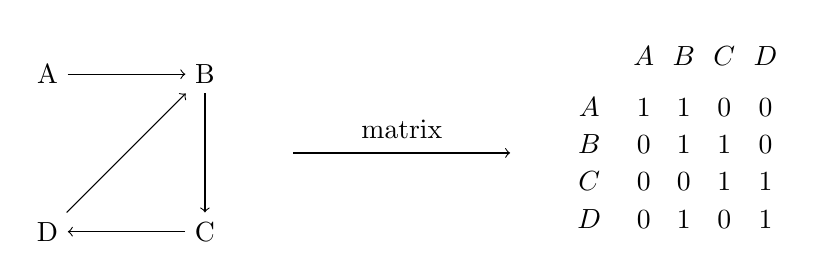
\begin{tikzpicture}[->]
    \node (a) at (1,3) {A};
    \node (b) at (3,3) {B};
    \node (c) at (3,1) {C};
    \node (d) at (1,1) {D};
    \draw (a) to (b);
    \draw (b) to (c);
    \draw (c) to (d);
    \draw (d) to (b);

    \node[matrix of math nodes] at (9, 2.2) {
          &[.5em] A & B & C & D\\[.5em]
        A & 1 & 1 & 0 & 0\\
        B & 0 & 1 & 1 & 0\\
        C & 0 & 0 & 1 & 1\\
        D & 0 & 1 & 0 & 1\\
    };
    \node (h1) at (4,2) {};
    \node (h2) at (7,2) {};
    \draw (h1) to (h2);
    \node (h3) at (5.5,2.3) {matrix};
\end{tikzpicture}
\end{center}
    \item Using repeated matrix multiplications\footnote{In this case, the
        formula for a matrix multiplication is $G'_{i,j} = \lor^n_{k=1} (G_{i,k}
    \land G_{k,j})$}, compute the $G'$
    \emph{composition matrix}; that is, the matrix where all the arrow
    compositions are present with the initial arrows. The composition matrix
    and the corresponding graph of the above example is the following:
\begin{center}
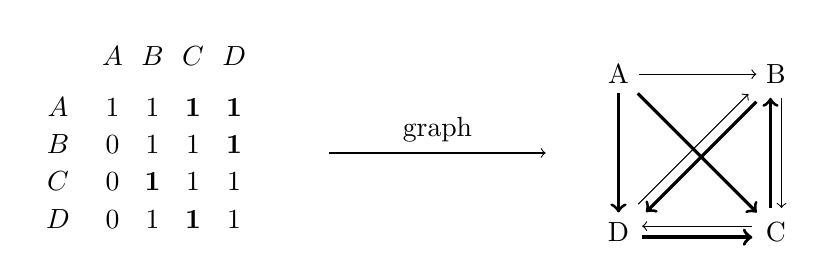
\begin{tikzpicture}[->]
    \node (a) at (7,3) {A};
    \node (b) at (9,3) {B};
    \node (c) at (9,1) {C};
    \node (d) at (7,1) {D};
    \draw (a) to (b);
    \draw[line width=0.4mm] (a) to (c);
    \draw[line width=0.4mm] (a) to (d);
    \draw (9.07,2.7) to (9.07,1.3);
    \draw[<-, line width=0.4mm] (8.93,2.7) to (8.93,1.3);
    \draw (8.7,1.07) to (7.3, 1.07);
    \draw[<-, line width=0.44mm] (8.7,0.93) to (7.3,0.93);
    \draw (7.25, 1.35) to (8.65, 2.75);
    \draw[<-, line width=0.4mm] (7.35, 1.25) to (8.75, 2.65);

    \node[matrix of math nodes] at (1, 2.2) {
          &[.5em] A & B & C & D\\[.5em]
        A & 1 & 1 & \mathbf1 & \mathbf1\\
        B & 0 & 1 & 1 & \mathbf1\\
        C & 0 & \mathbf1 & 1 & 1\\
        D & 0 & 1 & \mathbf1 & 1\\
    };
    \node (h1) at (3.2,2) {};
    \node (h2) at (6.2,2) {};
    \draw (h1) to (h2);
    \node (h3) at (4.7,2.3) {graph};
\end{tikzpicture}
\end{center}
    The composition matrix has an important property: it shows not just the
    direct dependencies of a node, but all the subsequent dependencies resulting
    from the direct dependencies. This can be used to efficiently find
    dependency cycles. The $i$th and $j$th nodes are in a cycle if and only if
    $G'_{i,j} \land G'_{j,i}$.
    \item Merge all the nodes that are in a dependency cycle.
\end{enumerate}

\subsubsection{The framework of type inference and type checking}

The type inference and type checking algorithms are stateful functions, which
mostly keep track of a dictionary called \verb$ReconcileEnv$, where the keys are
the indices of generic types, and the values are the types the generics should
be substituted with. Types related to this \verb$ReconcileEnv$ (i.e. types that
contain or can contain a generic index present in \verb$ReconcileEnv$) are part
of the same context, and therefore they have the type \verb$Type$ instead of
\verb$NormType$. 

There are two important invariant rules of \verb$ReconcileEnv$. First, there can
not be any keys that are present in any of the values as generic ids. Second,
if the values of two keys are different, then the keys have to be different as
well. These invariant rules help the type inference algorithm in a way that type
substitutions can be done in a single step.

There are two important helper functions:
\verb$reconcileTypesS$ and \\\verb$updateWithSubstitutions$. These functions
also use the same \verb$ReconcileEnv$ state.

\verb$reconcileTypesS$ is a helper function that can be given two types in the
same context. It returns either a new type that can be used in place of the two
given, or it returns an error, meaning that the two types can not be reconciled.
The function is used to assert type constraints, for example, when an \verb$I32$
is applied to an expression of type \verb$a -> b$, \verb$a$ can be reconciled
with \verb$I32$ to get \verb$I32 -> b$ as a new type for the function. As a
side-effect, the \verb$ReconcileEnv$ will contain the new key \verb$a$ with the
value \verb$I32$ to signify that the \verb$a$ generic type has to be replaced
with \verb$I32$ in subsequent calls to update. The \verb$reconcileTypesS$
function changes the \verb$ReconcileEnv$ context, therefore it is important to
update the related types with the changes using the
\verb$updateWithSubstitutions$ function.

The \verb$updateWithSubstitutions$ function takes a type and returns a possibly
different type. It reads the \verb$ReconcileEnv$ and if there are any generic
indices in the given type that also exist in the dictionary as keys, it
substitutes the generic types in the given type with the values of the keys
found in the \verb$ReconcileEnv$. This function does not change the state,
therefore it is safe to use without requiring an update.

\subsubsection{Type inference}

The most important function related to type inference is \verb$inferFromExprS$.
It is a stateful function, that takes a list of already resolved definitions,
an expression, and either returns a type error, or a type with an additional
list of inferred types from the function parameters whose lambda expressions are
outside of the given expression. This function is run recursively on an
expression and its sub-expressions, where it can find variables that are
declared outside of the expression the function is called on. The function keeps
track of all variables and their inferred types in the state, where each new
variable is assigned a generic type with a unique id. When more information is
found related to the variable, the stored type is updated using the
\verb$reconcileTypesS$ function.

Type inference is run on every global definition in the source code in the order
in which there are no unresolved dependencies. Because cyclic dependencies can
occur in the code, all definitions in a cycle are type inferred at the same
time; therefore cycles need to be treated differently from regular definitions.
There are two different functions to handle the two cases: \verb$mkInfExprCycle$
and \verb$mkInfExprTree$. Note that regular definitions are named \emph{trees}
in the code. To complicate matters, especially in the case of cyclic
dependencies, type wishes need to be applied right after the type of a
definition is inferred, since it has an effect on the definitions depending on
it.

\verb$mkInfExprTree$ is a function that takes the list of already resolved
definitions, one still unresolved expression, and returns either an error if a
type error has occurred or the expression with the inferred type or applied type
wish. Internally, it infers the type with \verb$inferFromExprS$, checks if there
are any type wishes added to the definition, and runs the type checking
algorithm if there are any.

While \verb$mkInfExprTree$ only infers the type of a single global variable,
\verb$mkInfExprCycle$ can infer any number of variable types. It takes the list
of already resolved definitions, a list of unresolved definitions, and it
returns either an error, if there are any, or a list of resolved definitions.
Internally, it walks the given list of to be inferred definitions and runs
\verb$inferFromExprS$ on each variable. After this, the type information
computed by the inference of the definitions on each other is taken into
account. Then all types are updated with \verb$updateWithSubstitutions$. After
the updating step, the type wishes can checked and substituted.

\subsubsection{Type checking}

Type checking is a comparatively small part of the type inference algorithm. It
can be understood as a stricter algorithm for type reconciliation. A type check
succeeds when two conditions are met: 
\begin{itemize}
    \item The type wish and the inferred type can be reconciled.
    \item The type wish is stricter than the inferred type.
\end{itemize}
Because of this, the function \verb$reconcileTypesS$ and \verb$checkTypeS$
(i.e., the function used for type checking) have a lot in common. The two main
differences are that \verb$checkTypeS$ does not substitute generic types that
originate from the type wish, and \verb$checkTypeS$ returns a unit on success.

\subsection{Code Generation}

\begin{figure}[ht]
\includegraphics[width=\textwidth]{code-generator.diag.pdf}
\centering
\caption{Module imports related to the Code Generator}
\end{figure}
\subsubsection{Pre-processing}

After all the semantic checks are completed, the code generation process can
start. The Code Generator needs to turn the representation of the code used in
the Semantic Analyzer into the more usable representation of the Code Generator.
This process does two main things:
\begin{itemize}
    \item All type information is discarded as the program is proven to be
        type-safe.
    \item Lambdas are represented with closures and closures acquire a
        \verb$depth$ value which is used to determine the number of captured
        values inside the closure.
\end{itemize}

\subsubsection{Garbage collection}

In the C source code that the Code Generator generates, there are five different
types of objects: Closures, Literals, Sums, Products, and Units. All of them
will be discussed in the later sections. All objects occupy memory on the heap,
which has to be allocated and deallocated manually. To simplify the LC language,
there is a garbage collector built into its runtime which can automatically
allocate and deallocate memory for objects. 

The garbage collector employs a simple mark-and-sweep algorithm. All objects
have a boolean flag indicating whether there is a pointer on the stack pointing
to them. This flag is managed by the generated code, and is used by the garbage
collector. Additionally, objects are stored in a linked list for easier access.
When the garbage collector is invoked, it walks the linked list storing all the
objects and if one of them has the stack flag turned on, it recursively walks
the object and the objects it refers to and marks them with a separate flag.
Once the whole linked list is walked, the garbage collector walks the list
again, discarding the objects that are not marked.

All objects can be cast to \verb$gc_type$. \verb$gc_type$ is a structure that
has the same memory layout for its garbage collection information as any other
object, however it does not have any other fields specified. \verb$gc_type$ is
used as a generic type in the garbage collector in order to more efficiently
manage objects.

All objects including \verb$gc_type$ share a common field called
\verb$gc_data$. It is a structure that holds all information necessary for
garbage collection: linked list primitives, object size and kind, the marker
flag, and the stack flag.

The stack flag is used to determine if an object is referenced directly from the
execution stack. Such objects, and objects referred to by objects on the stack
are considered to be in-use and therefore they are not freed by the garbage
collector. Managing the stack flag is the responsibility of the generated code.
When an object is in scope, its stack flag should be turned on, and when it goes
out of scope, its stack flag should be turned off. The two functions in the
program runtime that set and unset the stack flag are \verb$gc_set_stack$ and
\verb$gc_unset_stack$.

\subsubsection{Closures}

Closures are objects in the generated C source code that represent a function
(or lambda). They have two\footnote{All objects include the field
\texttt{gc\_data}, however it is not counted here, as it is not necessary for a
closure to function.} fields: \verb$clfunc$ and \verb$captures$. \verb$clfunc$
holds a function pointer, while \verb$captures$ is a variable length array
holding a number of captured values to be used when \verb$clfunc$ is called.

All \verb$clfunc$ function pointers take two pointers as arguments. Their first
argument should always point to the closure object while their second argument
should always point to the parameter the closure (or lambda) is being called
with.
\vspace{1em}
\\\noindent\begin{minipage}{\textwidth}
\begin{lstlisting}
void* cl_1_clfunc(closure* self, void* param) {
    // the code generated for the lambda expression body
}
\end{lstlisting}
\end{minipage}

Alongside \verb$clfunc$, all closures have a variable length array that holds
pointers to the objects the closure captures. These objects can be used in the
body of the \verb$clfunc$ call, to reference the values that are created outside
of the lambda definition.

\begin{lstlisting}
typedef struct {
    cl_func_t clfunc;
    void* captures[];
} closure;
\end{lstlisting}

Having the function pointer in the structure of the object makes it simple to
call a closure during runtime. When a closure is called, its \verb$clfunc$ field
is used in the following way:
\begin{lstlisting}
void* cl_param = some_other_function();
void* cl_ret = cl->clfunc(cl, cl_param); 
\end{lstlisting}
\textbf{Note:} The above code listing does not manage the stack flag of the
created objects. That part of the code has been omitted for simplicity.

As an example, the \verb$test$ definition of the following LC code
\begin{lstlisting}
a := <some definition>
b := <some definition>
test := a b
\end{lstlisting}
would compile to
\begin{lstlisting}
void* test_func() {
    closure* v1 = a_func();
    void* v2 = b_func();
    void* v3 = v1->clfunc(v1, v2);
    return v3;
}
\end{lstlisting}
Note that because global definitions are not necessarily lambdas, to call them,
one needs to postfix \verb$_func$ to the name of the global definition, and call
it as a function with no arguments.


\subsubsection{Literals} % todo: assignment

While closures represent functions, literal objects stand for primitive values
in the generated code. The only field alongside \verb$gc_data$ in their
structures are \verb$data$. It is a variable length \verb$char$ array that can
be sized according to the size of the data type contained in the object. This
approach allows literals to only consume the memory necessary, with the drawback
of having to do pointer casts to be able to read and write to this field.

\subsubsection{Sums}

Sum objects object represent an element of a Sum type in the LC language. They
can contain an object that is one of two different types. Internally, sum
objects store a pointer to the stored object named \verb$data$ as well as a
boolean flag indicating which type the stored object is the element of with the
name \verb$kind$.

\subsubsection{Tuples}

Tuple objects are similar to sums. While sums store only a single object, tuples
store two. The structure of a tuple object has a \verb$data_1$ and a
\verb$data_2$ field; both of them are pointers to the first and second stored
object respectively.

\subsubsection{Unit}

A unit object does not store any data besides garbage collection information,
and therefore there is no dedicated structure definition for units, only
\verb$gc_type$ is used. 

\subsubsection{A note on the Empty type}

While the Empty type is a valid type in the LC language, it is not necessary to
implement it into the generated C code. It is impossible to create an instance
of this type, and therefore functions on such an instance are unnecessary to
implement.

\subsubsection{If-expressions} % todo

\subsubsection{The standard library}

The standard library defines types and definitions for functions that are
available to the programmer by default. These functions provide a way to execute
C library calls, construct primitive types, and run basic operations on
primitive types.

The standard library is a list of entries. Each entry consists of a name, a type
definition used in the Semantic Analyzer, and a function that can be used to
generate the C source code for that standard library definition. In this
subsection, the process of generating C source for a definition is discussed.

The type definition of C source generators of an entry is
\begin{lstlisting}
(Int -> Writer a String) -> Writer a [String]
\end{lstlisting}
where \verb$(Writer a)$ is a monoid. It is a function that can be given a
function parameter that is used to generate variable names in a flexible way by
allowing an arbitrary type \verb$a$ to be retained after every call to the
parameter function. This method of using a \verb$Writer$ allows, for example, to
keep a record of the integer values the parameter function was called with,
which is used to determine how many parameters a standard library definition
requires.

Once the number of parameters necessary for a standard library function to work
is determined, the Code Generator generates several closures that gather the
parameters, (i.e., for each parameter, one closure is generated which captures
the given parameter and returns a closure that captures the next parameter
etc.). The body of the last closure function is filled in with the C code
returned by the generator function from the Standard Library.

The generator function in the Standard Library returns a 
\verb$Writer a [String]$. \verb$a$ can be used arbitrarily, while the
\verb$[String]$ holds the lines for the actual C code to be inserted. It is
expected that all lines in the list are postfixed with a semi-colon (\verb$;$)
and the last line to be prefixed with a \verb$return$ keyword.

As an example, the standard library definition of the \verb$cons$ function is
the following:
\lstset{numbers=left}
\begin{lstlisting}
( "cons",
  g 1 `to` T.ListType (g 1) `to` T.ListType (g 1),
  \w ->
    sequence
      [ p "sum* list = new_sum()",
        p "list->gc_data.isInStackSpace = 1",
        p "list->kind = 1",
        p "product* list_internal = new_product()",
        p "list_internal->gc_data.isInStackSpace = 1",
        p "list_internal->data_1 = " <> w 1,
        p "list_internal->data_2 = " <> w 2,
        p "list->data = list_internal",
        p "list->gc_data.isInStackSpace = 0",
        p "list_internal->gc_data.isInStackSpace = 0",
        p "list"
      ]
)
\end{lstlisting}
Lines 1 and 2 define the name and type of the \verb$cons$ function, while the
rest of the lines define the generator function. \verb$p$ is a shorthand for
\verb$pure$ to turn simple strings into \verb$(Writer a String)$ elements, while
\verb$w$ is the function that generates the variable names. The \verb$(<>)$
operator is used to concatenate the writers, and \verb$sequence$ is used for
simpler code, as it is easier to define a \verb$[Writer a b]$ element and turn
it into \verb$Writer a [b]$ than to define a \verb$Writer a [b]$ element
directly.

Writing standard library definitions in the above way abstracts away the details
of how closures are used to gather arguments, thereby reducing the size of the
Standard Library module and allowing the programmer to focus on the definition.

\subsection{Tests}

To validate that the compiler is working as expected, automated tests are used.
There are two types of tests for \verb$lcc$.
\begin{itemize}
    \item \textbf{Unit tests} are designed to focus on single parts of the program.
        They are used to test small but non-trivial features.
    \item \textbf{End-to-end tests} are designed to test every part of the
        system, (i.e. parsing, syntax checking, semantics checking, and code
        generation). 
\end{itemize}
Note that the following Haskell dependencies are required to compile and run
tests:
\begin{itemize}
    \item \verb$hspec$ is the testing framework.
    \item \verb$hspec-expectations$ is required for some utility functions.
    \item \verb$process$ is used to run \verb$gcc$, \verb$valgrind$, and the
        compiled binary.
    \item \verb$temporary$ is used to create temporary directories to store
        compilation results.
    \item \verb$QuickCheck$ is used for some random tests.
\end{itemize}
At the time of writing, all tests are passing.

\subsubsection{Unit tests}

Unit tests are divided into four categories: syntactic analyzer tests, semantic
analyzer tests, dependency list tests, and type tests. The unit tests can only
pass if all tests from all categories pass.

\subsubsection{End-to-end tests}

End-to-end tests are used to check every step of the compilation. They use
example programs written in a way to invoke specific features of the language,
thereby allowing them to be validated. End-to-end tests use the system installed
\verb$gcc$ and \verb$valgrind$ to also check the resulting binary of an example
program. These tests can only pass if
\begin{itemize}
    \item The program can be compiled by \verb$lcc$.
    \item The generated code can be compiled by \verb$gcc$ without warnings.
    \item The resulting binary runs correctly, and produces the expected result.
    \item During execution of the resulting binary, there are no memory errors
        detected by \verb$valgrind$.
\end{itemize}
\textbf{Note:} Some tests test for compilation errors. Those tests pass if there
\emph{is} a compilation error.

\subsection{The Utility module}

There is a Utility module imported into most other modules. The Utility module
defines utility functions and data-types that are either not specific to any module, or they
are used in more than one modules. (e.g. \verb$State$ is used in the Semantic
Analyzer and the Code Generator, however it is not specific to either of the two
modules.)

\end{document}
